Let us recall the definition of Steiner symmetrization. Write \(\R^n = \R^{n-1}\times \R\) with coordinates \(x=(z,t)\), \(z \in \R^{n-1}\), \(t=x_n \in \R\). Let \(E \subset \R^n\) and fix a unit vector \(v\in \R^n\). For every \(z \in \langle v \rangle^\perp= \R^{n-1}\), consider the \emph{\(v\)-vertical \(z\)-slice}
\[
    E_z^v \coloneq \{ t \in \R \colon z+tv \in E\} \subset \R.
\]
The \emph{Steiner symmetrization of \(E\) with respect to the direction \(v\)} is the set
\[
    S_v(E) \coloneq \left\{ z+tv\in \R^n= \langle v\rangle^\perp \oplus \langle v\rangle \colon |t| < \frac{1}{2}\Leb^1(E_z^v)\right\}.
\]
By Fubini's theorem, \(|S_v(E)|=|E|\). It is also quite easy to prove that
\[
    \diam(S_v(E)) \le \diam(E).
\]
In what follows, we will always identify \(\langle v \rangle^\perp = \R^{n-1}\) with a suitable change of coordinates, that is, we take \(v = e_n\). 

\begin{prop}[Slicing perimeter by lines]\label{prop: slicing}
    Let \(E \subset \R^n\) be a Lebesgue measurable set with \(|E|<\infty\) and \(P(E)<\infty\), and fix a unit vector \(v \in \R^n\). Then, 
    \begin{equation*}
        \int_{\R^{n-1}} P(E_z^v) \dif z \le P(E).
    \end{equation*}
    and in particular the \(v\)-vertical \(z\)-slice \(E_z^v\) is a set of finite perimeter in \(\R\) for a.e. \(z \in \R^{n-1}\).
\end{prop}
\begin{proof}
    Write \(E_z=E_z^v\). Fix a mollifier \(\rho \in C^\infty_c(B_1)\) and let \(u_\eps \coloneq \chi_E \star \rho_\eps\), so that
    \(u_\eps \to \chi_E\) and 
    \begin{equation}\label{eq: P(E)=lim_eps int nabla u_eps}
        P(E) = \lim_{\eps \to 0} \int_{\R^n} |\nabla u_\eps|\dif x.
    \end{equation}
    
    By Fubini's theorem,
    \[
        \int_{\R^{n-1}} \int_\R |u_\eps(z,t)-\chi_{E_z}(t)| \dif t \dif z = \int_{\R^n} |u_\eps-\chi_E| \dif x \to 0
    \]
    since \(u_\eps \to \chi_E\) in \(L^1\), so there exists a sequence \(\eps_h \searrow 0\) such that
    \[
        u_h(z,\cdot) \coloneq u_{\eps_h}(z,\cdot) \to \chi_{E_z} \qquad \text{for a.e. }z \in \R^{n-1}.
    \]
    By the lower semicontinuity of the total variation,
    \[
        P(E_z) \le \liminf_{h\to \infty} \int_\R \left|\de_t u_h(z,t) \right| \dif t \le \liminf_{h\to \infty} |\nabla u_h(z,t)|\dif t,
    \]
    and by Fatou's lemma, Fubini's theorem and \eqref{eq: P(E)=lim_eps int nabla u_eps}, we get
    \[
    \begin{aligned}
        \int_{\R^{n-1}} P(E_z) \dif z &\le \int_{\R^{n-1}} \left(\liminf_{h\to \infty} \int_\R |\nabla u_h(z,t)|\dif t\right) \dif z \\
        &\le \liminf_{h \to \infty} \int_{\R^{n-1}} \int_\R|\nabla u_h(z,t)| \dif t \dif z \\
        &= \lim_{h \to \infty} |\nabla u_h| \dif x = P(E),
    \end{aligned}
    \]
    as required.
\end{proof}


\begin{thm}[Steiner inequality]\label{thm: steiner inequality}
    Let \(E\subset \R^n\) be a set with \(|E|<\infty\) and finite perimeter \(P(E)<\infty\). Then for every unit vector \(v \in \R^n\)
    \begin{equation*}
        P(S_v(E)) \le P(E),
    \end{equation*}
    and the equality holds if and only the \(z\)-slice \(E_z^v\) is an interval for a.e. \(z \in \R^{n-1}\). 
\end{thm}

\begin{proof}
    Without loss of generality, assume that \(v=e_n\) and denote \(E_z=E_z^v\), \(E^s \coloneq S_{e_n}(E)\). We divide the proof in three steps.
    
    \emph{Step 1}. Assume that \(E\) is a bounded set with polyhedral boundary \(\de E\), and that the outer unit normal to \(E\) (defined \(\Haus^{n-1}\)-a.e. on \(\de E\)) is never orthogonal to \(e_n\). In particular, \(P(E)<\infty\) and \(|D\chi_E| = \Haus^{n-1}\resmes \de E\). Let \(G\) be the projection of \(E\) on \(\R^{n-1}\), or equivalently
    \[
        G= \{ z \in \R^{n-1} \colon \Leb^1(E_z)>0\}.
    \]
    Then in the definition of set with polyhedral boundary, we can always take \(T\) to be a translation, so there exist a finite partition \(\{G_h\}_{h=1}^M\) of \(G\) made of \((n-1)\)-polyhedral sets and affine functions 
    \[
        v_h^1, u_h^1, \dots, v^{N(h)}_h, u_h^{N(h)} \colon \R^{n-1} \to \R,
    \]
    such that 
    \begin{equation*}
    \begin{aligned}
        \de E &= \bigcup_{h=1}^M \bigcup_{k=1}^{N(h)} \Gamma(u_h^k,G_h) \cup \Gamma(v_h^k,G_h) \\
        E &= \bigcup_{h=1}^M \left\{(z,t) \in G_h \times \R \colon t \in \bigcup_{k=1}^{N(h)}(v_h^k(z), u_h^k(z))\right\}.
    \end{aligned}
    \end{equation*}

    \begin{figure}[ht]
		\centering
		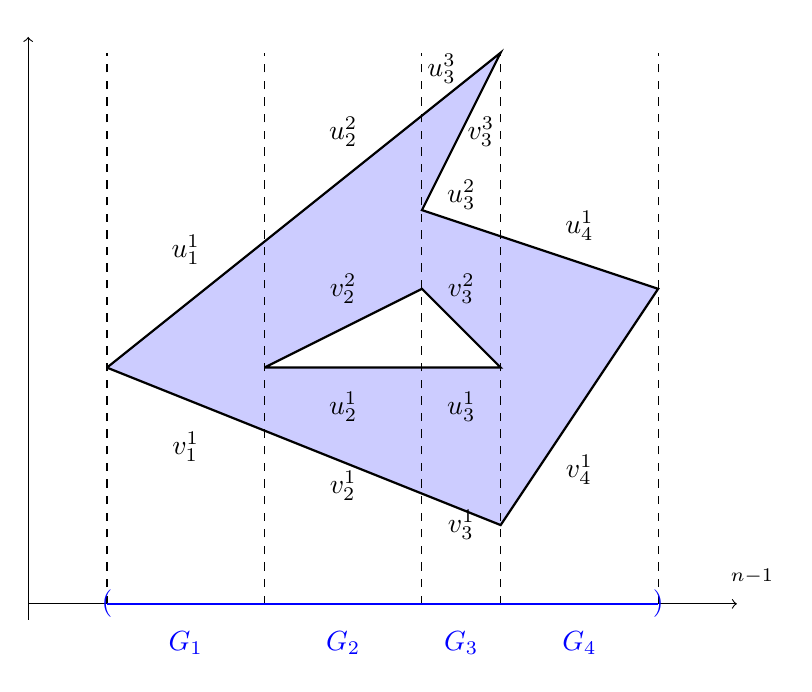
\begin{tikzpicture}
		%\draw[help lines] (-3,-3) grid (5,4);
        \draw [->](-4,-3) -- (5,-3);
        \node at (5.2,-2.7){\(\R^{n-1}\)};
        \draw [->](-4,-3.2) -- (-4,4.2);
        \node at (-3.7,4.2){\(\R\)};

        \fill[blue, opacity=0.2] (-3,0) -- (2,4)--(1,2)--(4,1)--(2,-2)--(-3,0);
        \draw[thick] (-3,0) -- (2,4)--(1,2)--(4,1)--(2,-2)--(-3,0);
        \draw[thick, fill=white] (-1,0)--(1,1)--(2,0)--(-1,0);
        \draw[dashed] (-3,-3)--(-3,4);
        \draw[dashed] (-1,-3)--(-1,4);
        \draw[dashed] (1,-3)--(1,4);
        \draw[dashed] (2,-3)--(2,4);
        \draw[dashed] (4,-3)--(4,4);
        
        \draw[thick, blue] (-3,-3)--(4,-3);
        \node[blue] at (-3,-3){\((\)};
        \node[blue] at (4,-3){\()\)};
        \node[blue] at (-2,-3.5){\(G_1\)};
        \node[blue] at (0,-3.5){\(G_2\)};
        \node[blue] at (1.5,-3.5){\(G_3\)};
        \node[blue] at (3,-3.5){\(G_4\)};

        \node at (-2,-1){\(v_1^1\)};
        \node at (-2,1.5){\(u_1^1\)};

        \node at (0,-1.5){\(v_2^1\)};
        \node at (0,-0.5){\(u_2^1\)};
        \node at (0,1){\(v_2^2\)};
        \node at (0,3){\(u_2^2\)};
    
        \node at (1.5,-2){\(v_3^1\)};
        \node at (1.5,-0.5){\(u_3^1\)};
        \node at (1.5,1){\(v_3^2\)};
        \node at (1.5,2.2){\(u_3^2\)};
        \node at (1.75,3){\(v_3^3\)};
        \node at (1.25,3.8){\(u_3^3\)};

        \node at (3,-1.3){\(v_4^1\)};
        \node at (3,1.8){\(u_4^1\)};
        
		\end{tikzpicture}
        \caption{Notation in step 1 of the proof of Theorem~\ref{thm: steiner inequality}.}
        \label{fig: polyhedral set}
	\end{figure}
    
    With this notation,
    \begin{equation}\label{eq: polyhedral perimeter}
    \begin{aligned}
        P(E) &= \Haus^{n-1}(\de E) = \sum_{h=1}^M\Haus^{n-1}(\de E \cap G_h \times \R) \\
        &= \sum_{h=1}^M \int_{G_h}\sum_{k=1}^{N(h)} \left( \sqrt{1+ |\nabla v_h^k|^2} + \sqrt{1+ |\nabla u_h^k|^2} \right)\dif z.
    \end{aligned}
    \end{equation}    
    For every \(z \in \R^{n-1}\),
    \[
        E_z = \left\{\begin{aligned}
            &\bigcup_{k=1}^{N(h)}(v_h^k(z), u_h^k(z))&& \text{ if }z \in G_h,\\
            &\ \varnothing &&\text{ if }z \in \R^{n-1}\setminus G
        \end{aligned} \right.
    \]
    and, if we set \(m(z)=\Leb^1(E_z)\) for every \(z \in \R^{n-1}\),
    \begin{equation}\label{eq: m(z)}
        m(z) \coloneq \Leb^1(E_z) = \left\{\begin{aligned} 
        & \sum_{k=1}^{N(h)} u_h^k(z)-v_h^k(z) && \text{ if }z \in G_h,\\
        & \ 0 &&\text{ if }z \in \R^{n-1}\setminus G.
        \end{aligned} \right.
    \end{equation}
    Observe that \(m \colon \R^{n-1} \to \R\) is affine on each \(G_h\). Therefore,
    \[
        E^s = \{ (z,t) \in \R^{n-1}\times \R \colon |t| < m(z)/2\}
    \]
    is a bounded set with polyhedral boundary, so in particular it has finite perimeter and \(|D\chi_{E^s}|= \Haus^{n-1}\resmes \de E^s\). By the area formula,
    \begin{equation}\label{eq: symmetrized polyhedral perimeter}
    \begin{aligned}
        P(E^s) &= \Haus^{n-1}(\de E^s) = 2 \int_G \sqrt{1+ \left|\frac{1}{2} \nabla m \right|^2} \dif z \\
        &= \sum_{h=1}^M\int_{G_h} \sqrt{4+ |\nabla m|^2} \dif z
    \end{aligned}
    \end{equation}

    By \eqref{eq: m(z)} and the convexity of the function \(z \mapsto \sqrt{1+|z|^2}\), for every \(h=1,\dots, M\)
    \begin{align*}
        \sum_{k=1}^{N(h)} \sqrt{1+|\nabla v_h^k|^2} + \sqrt{1+|\nabla u_h^k|^2} &\ge 2\sum_{k=1}^{N(h)} \sqrt{ 1+ \left|\frac{\nabla u_h^k-\nabla v_h^k}{2}\right|^2} \\
        &= 2N(h)\sum_{k=1}^{N(h)} \frac{1}{N(h)} \sqrt{ 1+ \left|\frac{\nabla u_h^k-\nabla v_h^k}{2}\right|^2}\\
        &\ge 2N(h) \sqrt{ 1+ \left|\sum_{k=1}^{N(h)} \frac{1}{N(h)}\frac{\nabla u_h^k-\nabla v_h^k}{2}\right|^2}\\
        &= \sqrt{4N(h)^2+|\nabla m|^2}.
    \end{align*}
    Therefore, by \(\eqref{eq: polyhedral perimeter}\) and \(\eqref{eq: symmetrized polyhedral perimeter}\), 
    \begin{equation}\label{eq: P(E^s)<(int)<P(E)}
        P(E^s) \le \sum_{k=1}^{N(h)} \int_{G_h} \sqrt{4N(h)^2+|\nabla m|^2} \dif z \le P(E).
    \end{equation}

    We have just found that
    \begin{align*}
        P(E)-P(E^s) &\ge \sum_{N(h)\ge 2} \int_{G_h} \left(\sqrt{4N(h)^2+|\nabla m|^2} - \sqrt{4+|\nabla m|^2} \right)\dif z\\
        &= \sum_{N(h)\ge 2} \int_{G_h} \frac{4(N(h)^2-1)}{\sqrt{4N(h)^2+|\nabla m|^2} + \sqrt{4+|\nabla m|^2}}\dif z\\
        & \ge \sum_{N(h)\ge 2} \int_{G_h} 2 \frac{1}{\sqrt{4N(h)^2 + |\nabla m|^2}} \dif z.
    \end{align*}
    If
    \[
        D \coloneq \{ z \in \R^{n-1} \colon E_z \text{ is not an interval}\} = \bigcup_{N(h)\ge 2} G_h,
    \]
    then by Cauchy-Schwarz inequality and \eqref{eq: P(E^s)<(int)<P(E)},
    \begin{equation}\label{eq: estimate on D}
        \begin{aligned}
            2\Leb^{n-1}(D)^2 &= 2 \left( \sum_{N(h)\ge 2}\int_{G_h} \frac{(4N(h)^2+|\nabla m|^2)^{1/4}}{(4N(h)^2+|\nabla m|^2)^{1/4}} \right)^2 \\
            &\le P(E) (P(E)-P(E^s)).
        \end{aligned}
    \end{equation}
    
    \emph{Step 2}. Now let \(E \subset \R^n\) with \(|E|<\infty\) and \(P(E)<\infty\). By Theorem~\ref{thm: polyhedral approximation} there exists a sequence of bounded sets \(E_h\) with polyhedral boundary such that
    \[
        E_h \to E, \qquad P(E_h) \to P(E).
    \]
    Note that we can assume that the outer unit normal of \(\de E_h\) is never orthogonal to \(e_n\). Indeed, this is an ‘‘open condition'', so if it happens that the unit normal of \(\de E_h\) is orthogonal to \(e_n\), we only need to rotate slightly \(\de E\). Doing smaller and smaller rotations as \(h \to \infty\), we still have that \(E_h \to E\) (while \(P(E_h) \to P(E)\) isn't affected by rotations). 

    For every \(h \in \N\), denote
    \[
        \begin{aligned}
            m_h(z) &\coloneq \Leb^1((E_h)_z), \quad m(z) \coloneq \Leb^1(E_z) \qquad \forall z \in \R^{n-1}\\
            G_h &\coloneq \{ z \in \R^{n-1} \colon m_h(z)>0\}, \qquad G\coloneq \{ z \in \R^{n-1} \colon m(z)>0\}\\
            D_h &\coloneq \{ z \in \R^{n-1} \colon (E_h)_z \text{ is not an interval}\}.
        \end{aligned}
    \]
    Applying step 1 to each \(E_h\), by \eqref{eq: P(E^s)<(int)<P(E)} and \eqref{eq: estimate on D} we get
    \begin{equation}\label{eq: step 1 to E_h}
        P(E_h^s) \le P(E_h), \qquad 2 \Leb^{n-1}(D_h)^2 \le P(E_h)(P(E_h)-P(E_h^s)).
    \end{equation}
    Moreover, by Fubini's theorem,
    \begin{equation*}
    \begin{aligned}
        |E\triangle E_h| &= \int_{\R^{n-1}} \Leb^1((E_h)_z \triangle E_z) \dif z \\
        &\ge \int_{\R^{n-1}}|m_h(z)- m(z)| \dif z = |E_h^s \triangle E^s|,
    \end{aligned}
    \end{equation*}
    so in particular \(E_h^s \to E^s\) and by lower semicontinuity
    \[
        P(E^s) \le \liminf_{h \to \infty} P(E_h^s) \le \lim_{h \to \infty} P(E_h) = P(E).
    \]
    Moreover,
    \begin{equation}\label{eq: G_h -> G, E_hz -> E_z}
        G_h \to G, \qquad (E_h)_z \to E_z \quad \text{ for a.e. }z \in \R^{n-1}
    \end{equation}
    By Proposition~\ref{prop: slicing} the vertical \(z\)-slices \((E_h)_z\) and \(E_z\) have finite perimeter for a.e. \(z \in \R^{n-1}\), thus by the lower semicontinuity of the perimeter
    \begin{equation}\label{eq: P(E_z) < liminf P(E_hz)}
        P(E_z) \le \liminf_{h \to \infty}P((E_h)_z).
    \end{equation}

    Now, assume that \(P(E)=P(E^s)\). Then, by \eqref{eq: step 1 to E_h}, \(\chi_{D_h} \to 0\) in \(L^1(\R^{n-1})\), so, up to passing to a subsequence, we have the pointwise limit
    \[
        \chi_{G}(z) = \lim_{h \to \infty}\chi_{G_h\setminus D_h}(z)
    \]
    for a.e. \(z \in \R^{n-1}\). By \eqref{eq: P(E_z) < liminf P(E_hz)},
    \[
        \chi_G(z)P(E_z) \le \liminf \chi_{G_h \setminus D_h}(z)P((E_h)_z) \qquad \text{ for a.e. } z \in \R^{n-1},
    \]
    therefore, by Fatou's lemma,
    \begin{equation*}
    \begin{aligned}
        \int_G P(E_z) \dif z & \le \int_{\R^{n-1}} \liminf \chi_{G_h \setminus D_h}(z)P((E_h)_z) \dif z\\
        &\le \liminf_{h \to \infty} \int_{G_h \setminus D_h}P((E_h)_z) \dif z\\
        &= 2 \liminf_{h \to \infty} \Leb^{n-1}(G_h \setminus D_h) \\
        &= 2 \Leb^{n-1}(G) \\
        &\le \int_G P(E_z) \dif z
    \end{aligned}
    \end{equation*}
    having used the 1-dimensional isoperimetric inequality in the last line, i.e., that \(P(E_z) \ge 2\) for a.e. \(z \in \R^{n-1}\). This implies that \(P(E_z)=2\) for a.e. \(z \in \R^{n-1}\), so, by the characterization of the equality in the 1-dimensional case, \(E_z\) is an interval for a.e. \(z \in \R^{n-1}\). 
\end{proof}

\begin{lemma}
    Let \(E\subset \R^n\) be a convex set with \(|E|<\infty\) and \(P(E)<\infty\), and let \(v\in\R^{n-1}\) a unit vector such that \(P(S_v(E))=P(E)\). Then there exists \(c \in \R\) such that \(E\) is equivalent to the translated \(S_v(E) + cv\).
\end{lemma}
\begin{proof}
    Assume without loss of generality that \(v=e_n\), and denote \(S_v(E)=E^s\). Since \(\Leb^n(\de E)=0\)\footnote{
    Indeed, without loss of generality assume that \(0 \in \mathring{C}\). Then by convexity, for every \(\eps>0\)
    \[  
        \de C \subset \left(\frac{1}{1-\eps}\mathring{C} \right) \setminus C.
    \]
    }, 
    we may assume that \(E\) is open. Then the projection \(G\subset \R^{n-1}\) is a convex set, and for every \(z \in G\), the vertical \(z\)-slice is equivalent to the open interval \((-v(z),u(z))\), where \(v,u \colon G \to \R\) are concave non negative functions, so in particular they are locally Lipschitz and \(E\) has Lipschitz boundary. By Rademacher's theorem, \(\nabla u\) and \(\nabla v\) are defined at a.e. \(z \in G\), so
    \begin{equation*}%\label{eq: P(E), P(E^s) convex case}
    \begin{aligned}
        P(E) &= \int_G \left( \sqrt{1+|\nabla u|^2} + \sqrt{1+|\nabla v|^2} \right) \dif z\\
        P(E^s) &= 2\int_G  \sqrt{1+\left| \frac{\nabla u + \nabla v}{2}\right|^2} \dif z
    \end{aligned}
    \end{equation*}
    since 
    \[  
        E^s = \left\{ (z,t) \in G \times \R \colon |t|< \frac{u(z)+v(z)}{2}\right\}.
    \]
    By the strict convexity of the function \(z \mapsto \sqrt{1+|z|^2}\),
    \[
        \sqrt{1+|\nabla u|^2} + \sqrt{1+|\nabla v|^2} \ge 2\sqrt{1+\left| \frac{\nabla u + \nabla v}{2}\right|^2}
    \]
    with equality if and only if \(\nabla u = \nabla v\). Hence, if \(P(E^s)=P(E)\), the equality holds almost everywhere and there must be that \(\nabla u = \nabla v\) a.e. in \(G\). Thus, there exists \(c \in \R\) such that \(u(z)-v(z)= c\) for a.e. \(z \in G\), which implies that 
    \[
    \begin{aligned}
        E&= \left\{ (z,t) \in G \times \R \colon -u(z)-c < t < u(z)\right\},\\
        E^s&= \left\{ (z,t) \in G \times \R \colon -u(z)-c/2 < t < u(z)+c/2\right\},
    \end{aligned}
    \]
    that is \(E= E^s + \frac{c}{2}e_n\).
\end{proof}

Recall that the density of \(E\) at a point \(x \in \R^n\) is
\[
    \Theta(E,x) \coloneq \lim_{r \to 0} \frac{|E \cap B_r(x)|}{\omega_n r^n}
\]
whenever it exists. It's easy to show that, whenever this limit exists, it's actually equal to
\begin{equation}\label{eq: density with cubes}
    \Theta(E,x)= \lim_{r \to 0} \frac{|E \cap Q^n(x,r)|}{2^nr^n}
\end{equation}
where
\[
    Q^n(x,r)= x+(-r,r)^n
\]
is the cube centered at \(x\) with side \(2r\). 

Observe that \(\Leb^n \resmes E= \chi_E \Leb^n\), so by Besicovitch differentiation theorem, 
\[
    \chi_E = \frac{\dif (\Leb^n \resmes E)}{\dif \Leb^n} = \Theta(E,\cdot)
\]
a.e. on \(\R^n\), that is,
\[
    \Theta(E,x)= \begin{cases}
        1 & \text{ a.e. }x \in E\\
        0 & \text{ a.e. }x \in \R^n \setminus E.
    \end{cases}
\]
In particular, \(E\) is equivalent to
\[
    E^{(1)} \coloneq \{ x \in \R^n \colon \Theta(E,x)=1\},
\]
the set of with density one points of \(E\). This will be the ‘‘good set'' to replace \(E\) with.

\begin{lemma}\label{lemma: density points and vertical sections}
    Let \(E \subset \R^n\) be a set of locally finite perimeter and suppose that \(E_z\) is equivalent to an interval for a.e. \(z \in \R^{n-1}\). Then \((E^{(1)})_z\) is an interval for every \(z \in \R^{n-1}\).
\end{lemma}
\begin{proof}
    Let \(z_0 \in \R^{n-1}\), and suppose that \(x_1=(z_0,t_1),x_2=(z_0,t_2) \in E^{(1)}\) for some \(t_1<t_2\), and fix \(t_0 \in (a,b)\). We have to prove that \(x_0=(z_0,t_0) \in E^{(1)}\), that is \(\Theta(E,x_0)=1\).

    Fix \(0<\eps< 1\), and for every \(t \in \R\), \(r>0\) denote \(I_r(t) = B_r(t)= (t-r,t+r)\). Since \(x_1,x_2 \in E^{(1)}\), \(\Theta(E,x)=\Theta(E,y)=1\), so by \eqref{eq: density with cubes} there exists \(\overline{r}>0\) such that for every \(r<\overline{r}\)
    \begin{equation}\label{eq: x_k density one}
        |E\cap Q^n(x_k,r)| \ge \left(1-\frac{\eps}{2}\right) 2^n r^n, \quad I_r(t_0)\cap I_r(t_k)=\varnothing \qquad k=1,2.
    \end{equation}
    Fix \(r<\overline{r}\) and for \(k=1,2\) denote by \(G_k\) the set of \(z \in Q^{n-1}(z_0,r)\) such that \(E_z\) is equivalent to an interval and \(\Leb^1(E_z \cap I_r(t_k))>0\). Since \(E_z\) is equivalent to an interval for a.e. \(z \in \R^{n-1}\), by Fubini's theorem
    \[
        |E \cap Q^n(x_k,r)| = \int_{G_k} \Leb^1(E_z \cap I_r(t_k)) \dif z \le 2r \Leb^{n-1}(G_k).
    \]
    Combining this with \eqref{eq: x_k density one},
    \[
        \Leb^{n-1}(G_k) \ge \left(1-\frac{\eps}{2}\right) 2^{n-1} r^{n-1}, \qquad k=1,2.
    \]
    Therefore, 
    \[
    \begin{aligned}
        \Leb^{n-1}(G_1\cap G_2) &= \Leb^{n-1}(G_1) +\Leb^{n-1}(G_2) - \Leb^{n-1}(G_1 \cup G_2) \\
        &\ge \Leb^{n-1}(G_1) +\Leb^{n-1}(G_2) - \Leb^{n-1}(Q^{n-1}(z_0,r))\\
        &\ge (1-\eps) 2^{n-1} r^{n-1}.
    \end{aligned}        
    \]
    Now let \(z \in G_1 \cap G_2\). Since \(E_z\) is equivalent to an interval and \(\Leb^1(E_z \cap I_r(t_k))>0\) for \(k=1,2\), by \eqref{eq: x_k density one} we have
    \[
        \Leb^1(E_z \cap I_r(t_0))=2r.
    \]
    Integrating this over \(G_1 \cap G_2\), we find
    \[
    \begin{aligned}
        |E\cap Q^n(x_0,r)| &\ge \int_{G_1\cap G_2} \Leb^1(E_z \cap I_r(t_0)) \dif z \\
        &= 2r \Leb^{n-1}(G_1 \cap G_2) \ge (1-\eps) 2^n r^n.
    \end{aligned}
    \]
    for every \(r<\overline{r}\). Since \(\eps>0\) was arbitrary,
    \[
        \lim_{r \to 0} \frac{|E\cap Q^n(x_0,r)|}{2^n r^n} = 1,
    \]
    which proves that \(x_0 \in E^{(1)}\). 
\end{proof}